\chapter{Analisi statica}

\section{Struttura binari}

\subsection{ELF}

\subsection{PE}
Potrebbero essere offuscati, come vedremo più avanti

\section{Capa: capabilities}
Includere anche il test su Colab con le statistiche.

\section{Yara: signature-based}
Sia per statici che in memoria dei processi.

Ora però usate solo per analizzare staticamente un file eseguibile.

\section{File offuscati}
Packed, installer, ... come li trattiamo?

Analisi rimandata alla parte dinamica, perché lì possiamo sfruttare altri strumenti di analisi integrati in Cuckoo, più potenti di quello che potremmo fare manualmente qui.

Ci basta avere i dati di ciò che stiamo trattando, ad esempio l'output in questo caso sarà del tipo:
\begin{code}
\captionof{listing}{Output CAPA su file packed}
\label{code:json_capa_packed}
\begin{minted}{json}
{
    "capa": {
        "format": "packed",
        "arch": "i386",
        "os": "windows"
    }
}
\end{minted}
\end{code}

Nessuna regola viene eseguita, perché \texttt{capa} non supporta questi formati per l'estrazione delle capabilities usando i propri strumenti integrati. \ref{code:json_capa_packed}

\section{Riconoscitore custom del tipo di file}
Partendo dalla necessità di velocizzare l'operazione di riconoscimento del file, in sostituzione dell'esecuzione del comando \texttt{capa -r anti-analysis} che può portare a richiedere diversi minuti a seconda del numero di funzioni presenti nel file, come visto in \textbf{FIGURA REF},
dobbiamo ricorrere a una diversa soluzione.

Dato che si tratta di un problema di enumerazione, non aveva senso andare a creare e mantenere un proprio riconoscitore di ogni possibile formato di un file. Ad esempio, già solo per quanto riguarda i file pacchettizzati, esistono tantissimi packer e tanti ne esisteranno in futuro.

Inoltre, spesso malware usano packer personalizzati, che hanno leggere differenze da quelli noti e si correrebbe il rischio di creare uno strumento poco efficace.
Per questi e altri motivi quali il tempo a disposizione, è stato scelto di usare come base uno strumento noto (\texttt{Detect-It-Easy}) per fare una prima analisi, affiancato da uno script Python custom che decide quali operazioni svolgere a seconda del tipo di file, va a fare il parsing del JSON dato in output e si integra nello script Bash creando un layer di astrazione col resto del workflow.
Infatti, nel caso servisse modificare lo strumento sottostante, sarebbe sufficiente adattare la traduzione dall'output specifico del tool al contratto stabilito col resto del programma per rendere seamless questa variazione, anche sostanziale.

Tuttavia, ci sono alcuni tipi che anche Detect-It-Easy fallisce a riconoscere, portando poi a un crash di capa quando eseguito.
Per questo motivo è stato creato un \textbf{custom detector}, scritto in Python, che implementa in maniera molto più efficiente e diretta, le sole regole di capa che riconoscono i file specifici su cui non è in grado di lavorare.

Di seguito possiamo osservare come funziona per dei tipi famosi di questi strumenti, ovvero il packer UPX e l'installer InnoSetup.
Sono state usate caratteristiche e regole note
\footnote{\url{https://github.com/mandiant/capa-rules/tree/e88db21de4d4cf9f7abec9177fab11240075036b/anti-analysis/packer}}
per eseguire la detection.

La lettura degli header del file PE sfrutta la libreria pefile per non eseguire l'intero parsing a mano dei byte degli header e non essere dipendenti da implementazioni native dell'OS come con l'uso dell'header \texttt{<windows.h>} in un programma C.

\begin{figure}[ht]
    \centering
    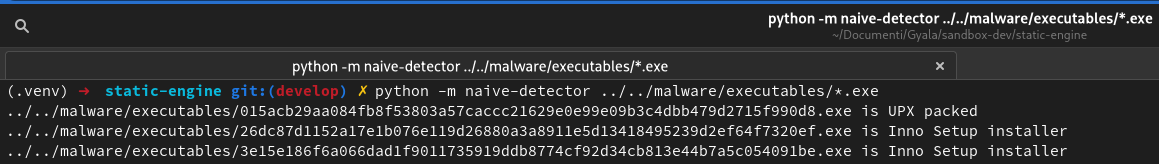
\includegraphics[width=\textwidth]{assets/custom_file_detector_output.png}
    \caption{Custom file detector output}
\end{figure}

\subsection{UPX}
Le regole più comuni
\footnote{\url{https://github.com/mandiant/capa-rules/blob/e88db21de4d4cf9f7abec9177fab11240075036b/anti-analysis/packer/upx/packed-with-upx.yml}}
per riconoscere UPX impongono di leggere le sezioni, e vedere se queste contengono \texttt{UPX0} o \texttt{UPX1}.

Facciamo una comparazione tra la regola capa per il rilevamento e il codice del riconoscitore.

\noindent\begin{minipage}{.35\textwidth}
       \begin{minted}{yaml}
features:
    - format: pe
    - or:
      - section: UPX0
      - section: UPX1
       \end{minted}
\end{minipage}
\begin{minipage}{.4\textwidth}
       \begin{minted}{python}
def is_upx(file_path):
    file_sections = get_section_names(file_path)
    upx_sections = [ "UPX0", "UPX1" ]
    for upx_section in upx_sections:
        if upx_section in file_sections:
            return True
    return False
       \end{minted}
\end{minipage}

\bigskip

Andando però a sfruttare la libreria Python per il parsing del file PE senza ricorrere a implementazioni native Windows:

\begin{minted}{python}
import pefile

def get_section_names(file_path):
    pe = pefile.PE(file_path)
    sections_set = {
        section.Name.decode().strip().strip('\x00')
        for section in pe.sections
    }
    pe.close()
    return sections_set
\end{minted}

\subsection{Inno-Setup Installer}
Con Inno-Setup, possiamo notare come sia ancora più semplice il riconoscimento. Infatti, non abbiamo bisogno di andare a vedere le sezioni, ma è sufficiente controllare la presenza di alcune stringhe statiche nel file.

Nuovamente, andiamo a paragonare la regola capa alla nostra implementazione:

\begin{minted}{yaml}
features:
    - and:
      - string: /^Inno Setup Setup Data \(/
      - string: /^Inno Setup Messages \(/
\end{minted}

\begin{minted}{python}
def is_innosetup(file_path):
    BUFFER_SIZE = 65536
    with open(file_path, 'br') as f:
        match_setup, match_messages = False, False
        buffer = f.read(BUFFER_SIZE)
        overlap = len(b'Inno Setup Setup Data (')

        while len(buffer) > overlap and (not match_setup or not match_messages):
            # Match inside current buffer
            if not match_setup and b'Inno Setup Setup Data (' in buffer:
                match_setup = True
            if not match_messages and b'Inno Setup Messages (' in buffer:
                match_messages = True
            
            # Read next buffer, allowing for overlap
            buffer = buffer[-overlap:] + f.read(BUFFER_SIZE)
    
    return match_setup and match_messages
\end{minted}

\subsection{Design scalabile e modulare}
Si nota immediatamente come una tale implementazione è poco scalabile e presenta numerose ridondanze da rimuovere.

Studiando le regole di interesse all'interno del repository GitHub \textit{capa-rules}, osserviamo come le regole siano principalmente di due categorie: basate su match di stringhe o basate su match di nomi di sezioni nel file eseguibile.

Da questa osservazione, elaboriamo la struttura del programma software di detection. Precisamente, decidiamo di strutturarlo in classi dove ogni regola è una classe a sé, e individuiamo le seguenti classi padre (figura \ref{fig:base_custom_static_analyzer_uml}):
\begin{itemize}
    \item \texttt{BaseRule} conterrà le logiche di base che possiede una regola, tra cui un getter per il nome e un metodo \texttt{match()}
    \item \texttt{StringRule} conterrà il codice unico per tutte le regole che basano il loro match sulla presenza di determinate stringhe all'interno del file, quindi la classe figlia dovrà solo fornire le stringhe da cercare e la logica di match (ad esempio: tutte le stringhe richieste devono essere state trovate = and logico; una sola stringa trovata è sufficiente = or logico)
    \item \texttt{SectionRule} analogamente a prima conterrà le procedure di estrazione delle sezioni dal file, con la logica di match nelle classi figlie, ossia le effettive regole.
\end{itemize}

Sempre al fine di ottimizzare i tempi di esecuzione di questo rilevamento statico sul file eseguibile,
andiamo a creare una classe wrapper sopra \texttt{pathlib.Path} che esporrà i metodi per leggere le sezioni, procedura lenta se ripetuta per ogni singola regola, e alcune altre funzioni di utilità come la rilevazione del tipo basilare di file (PE o ELF) eseguibile tramite l'ausilio di \texttt{libmagic}, la stessa che permette al comando \texttt{file} di operare.
Quindi da un lato è stata aumentata l'astrazione tra la business logic del programma e i dettagli implementativi delle librerie sottostanti, dall'altro possiamo aggiungere meccanismi di lazy-loading e caching di tali informazioni richieste.

\begin{figure}[H]
    \centering
    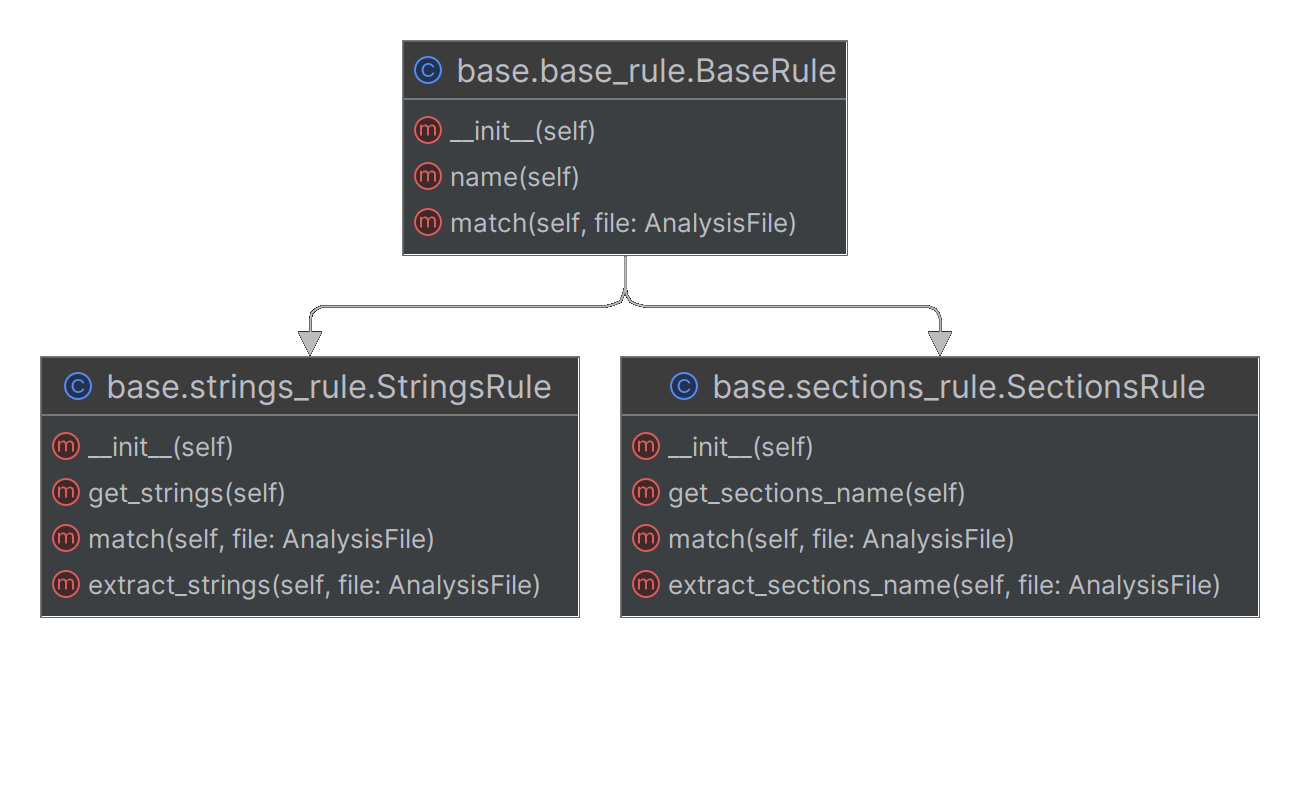
\includegraphics[width = 0.8\textwidth]{assets/base_custom_static_analyzer.png}
    \caption{Diagramma UML delle classi}
    \label{fig:base_custom_static_analyzer_uml}
\end{figure}

\begin{figure}[H]
    \centering
    \begin{minted}{python}
class InnoSetupDetector(StringsRule):
    def name(self) -> str:
        return 'executable/installer/inno-setup'

    def get_strings(self) -> list[bytes]:
        return [
            b'Inno Setup Setup Data (',
            b'Inno Setup Messages (',
        ]

    def match(self, file: AnalysisFile) -> bool:
        # && logic
        return len(self.extract_strings(file)) == len(self.strings)
    \end{minted}
    \caption{Regola di riconoscimento di InnoSetup, usando la nuova architettura}
    \label{fig:enter-label}
\end{figure}

\section{FLARE Floss}
Teoria: \url{https://github.com/mandiant/flare-floss/blob/master/doc/theory.md}

\section{Automazione su AWS}

\subsection{Scrittura dei parser}
Parser per capa e yara.

Parser dal file testuale, con schemini.

\subsection{Architettura serverless}
L'architettura è ben riassunta nel seguente diagramma, che andremo a spiegare:
\begin{figure}[htbp]
    \centering
    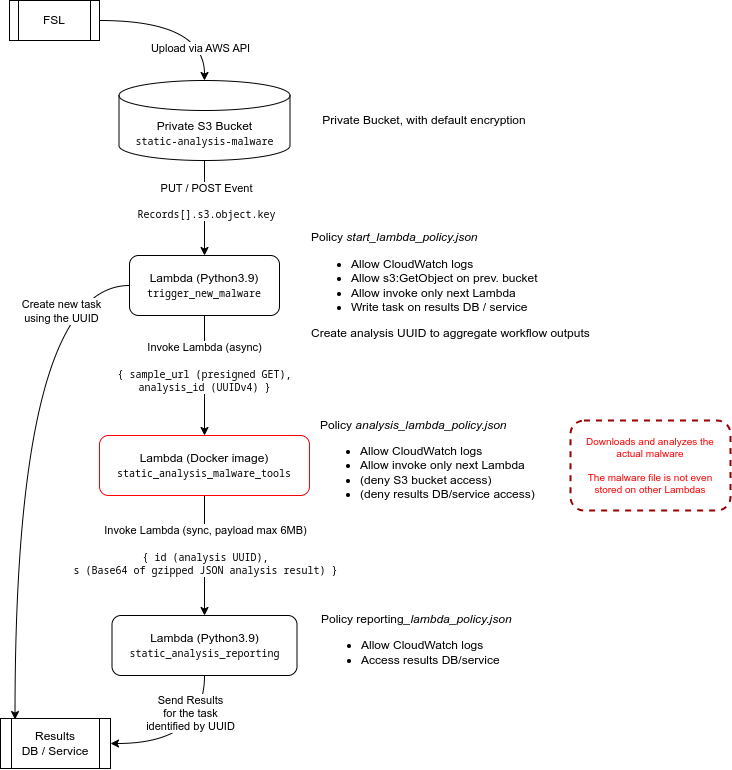
\includegraphics[width=\textwidth]{assets/aws_static_lambdas_architecture.png}
    \caption{Archittetura su AWS con i vari componenti coinvolti}
    \label{fig:aws_static_lambdas_architecture}
\end{figure}

\begin{figure}[htbp]
    \centering
    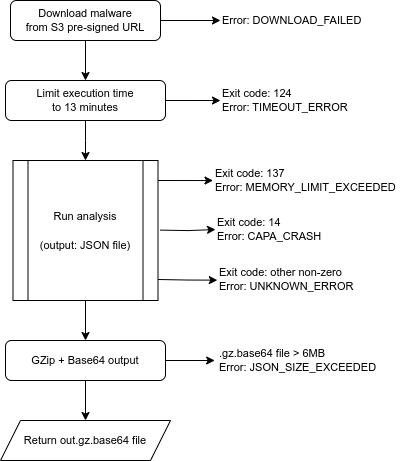
\includegraphics[width=0.75\textwidth]{assets/docker_static_analysis_flow.png}
    \caption{Workflow dell'analisi in \texttt{static\_analysis\_malware\_tools} e possibili errori}
    \label{fig:enter-label}
\end{figure}

\begin{figure}[htbp]
    \centering
    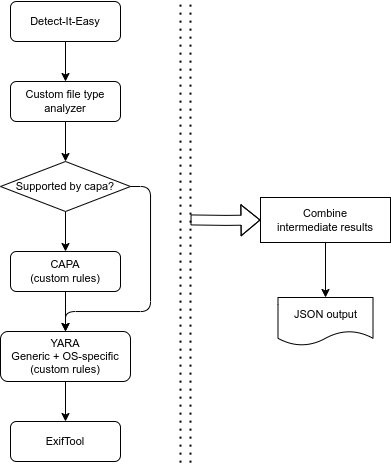
\includegraphics[width=0.75\textwidth]{assets/static_run_analysis_internal_tools.png}
    \caption{Workflow processo interno di \texttt{run\_analysis}}
    \label{fig:enter-label}
\end{figure}

\subsection{Creazione dell'immagine}
Prima era enorme (naive approach), poi ridotta sfruttando il multistage.

\begin{figure}[H]
    \centering
    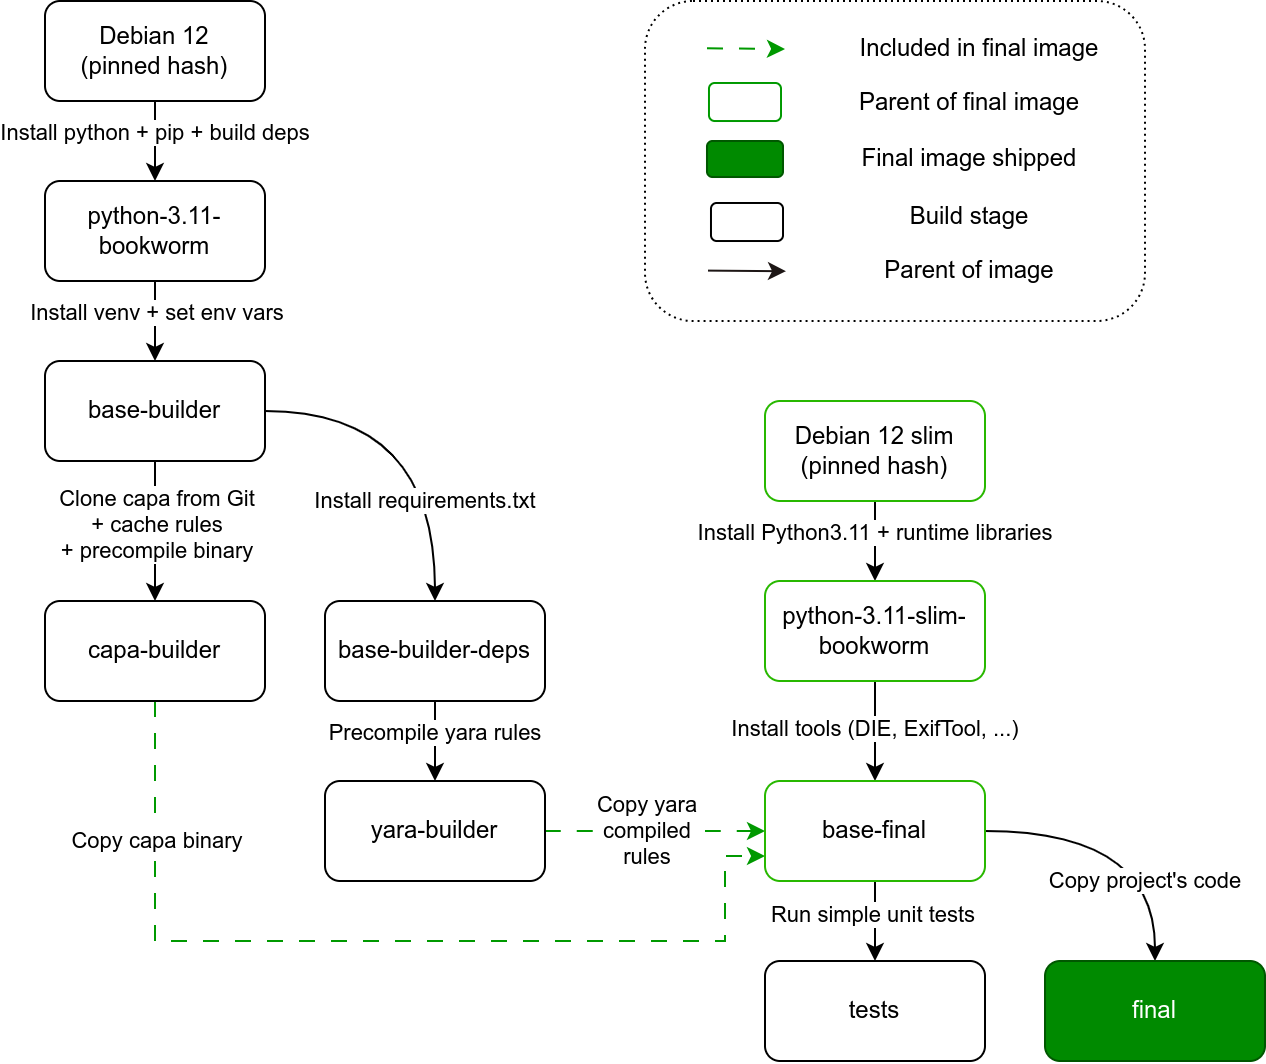
\includegraphics[width=\textwidth]{assets/dockerfile.png}
    \caption{Docker multi-stage build, con le immagini intermedie}
    \label{fig:static_dockerfile_multistage_build}
\end{figure}

Uso di CMD/ENTRYPOINT così da rendere l'immagine usabile sempre, che sia da URL o da cartella su cui itera.


Serve eseguirla su Lambda = serve rispettare la Runtime Interface!


\subsection{Deploy e hardening}
Sicurezza e varie policy (hardening)

\subsection{Limiti delle Lambda}

CPU time e memoria. Gestione degli errori (status 137 OOM).

\begin{figure}[H]
     \begin{subfigure}[b]{0.5\textwidth}
         \centering
         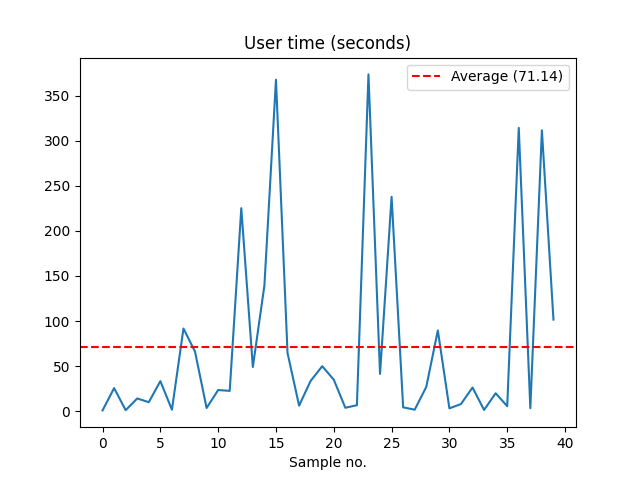
\includegraphics[width=\textwidth]{assets/static_analysis_exec_cpu_time.png}
         \caption{CPU}
         \label{fig:static_analysis_exec_cpu_time}
     \end{subfigure}
     \begin{subfigure}[b]{0.5\textwidth}
         \centering
         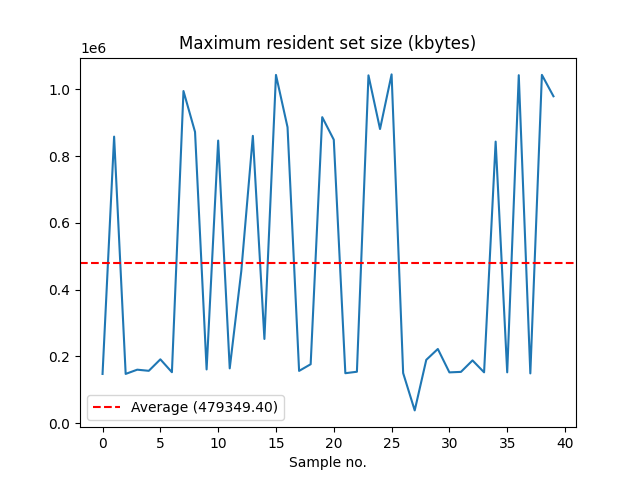
\includegraphics[width=\textwidth]{assets/static_analysis_exec_memory.png}
         \caption{Memoria}
         \label{fig:static_analysis_exec_memory}
     \end{subfigure}
     \label{fig_static_analysis_exec_stats}
     \caption{Uso delle risorse eseguendo analisi statica su malware reali presi a campione}
\end{figure}

6MB / 256KB in base a sync/async invocation.

\begin{figure}[H]
    \centering
    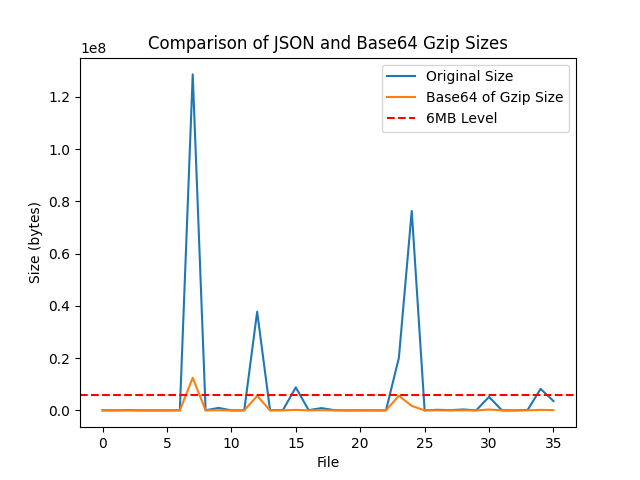
\includegraphics[width=0.6\textwidth]{assets/static_analysis_results_size.png}
    \caption{Dimensione del file di output originale e post-compressione gzip + base64}
    \label{fig:static_analysis_results_size}
\end{figure}

\subsection{Costi del servizio}
Le prossime analisi si baseranno sui seguenti parametri di riferimento forniti sulla base dello storico aziendale e delle aspettative di uso reale del servizio:
\begin{table}[H]
    \centering
    \begin{tabular}{|l|l|}
        \hline
        \textbf{Parametro}             & \textbf{Valore (al mese)}       \\ \hline
        Numero di sample da analizzare & 1.000.000                       \\
        Memoria media richiesta        & 512 MB (limite massimo: 1024MB) \\
        Tempi medio di esecuzione      & 70 secondi                      \\ \hline
    \end{tabular}
\end{table}

Inoltre, si sottolinea come i costi dei servizi AWS subiscano inflessioni nel tempo, per cui questa stima è sufficientemente valida al momento della scrittura di questo documento.

\begin{table}[H]
    \centering
    \begin{tabular}{|l|l|}
        \hline
        \textbf{Servizio}         & \textbf{Costo stimato (al mese)} \\ \hline
        S3 Bucket (standard tier) &                                  \\
        Lambda start              &                                  \\
        Lambda di analisi         &                                  \\
        Lambda di fine rapporto   &                                  \\ \hline
        Costo stimato totale      & € 750,00                         \\ \hline
    \end{tabular}
\end{table}

\section{Versioning}
Per il versioning, è stato creato un repository Git sul server GitLab aziendale.

Per ogni modifica viene creato un commit, come è standard.

Tuttavia, ci sono alcuni aspetti dell'organizzazione che ha senso sottolineare.

\subsection{Branch Naming Convention}
Per la gestione del repository,e in particolare i suoi branch, si seguono rigidamente queste convenzioni:
\begin{itemize}
    \item \texttt{main} è il branch principale dove deve essere presente solo codice finito e considerabile stabile a tutti gli effetti;
    \item \texttt{develop} è dove si tiene il codice che si considera usabile ma non ancora sufficientemente testato o pronto all'uso in produzioni così com'è - su questo branch infine è dove viene fatto il merge dei successivi branch più specifici;
    \item \texttt{feature/<feat-name>} è l'insieme di tutti i branch, originati da \emph{develop}, dove si lavora all'implementazione di una specifica funzione - ciò permette di mantenere il branch \emph{develop} funzionante, privo di funzioni non completamente realizzate, e diminuisce le interferenze tra chi sta lavorando sulla stessa codebase ma su funzioni distinte tra loro - e il prefisso \textbf{feature/} identifica chiaramente che si tratta di un branch dove si lavora solo ed esclusivamente su una sola funzionalità;
    \item \texttt{refactor/<ref-name>} invece rappresenta l'insieme dei branch dove si fa, con diversi gradi di complessità, refactoring del codice - ad esempio, nel progetto è stato realizzato un branch di refactoring per passare dall'uso di \texttt{os.path} al modulo Python \texttt{pathlib} per una maggiore usabilità
\end{itemize}

Infine, per un maggiore controllo, il merge dai branch secondari (\texttt{feature/} e \texttt{refactor}) vengono fatti attraverso l'uso di \emph{Merge Request} (o \emph{Pull Request}, a seconda che si usa la nomenclatura di GitLab o di GitHub).
In questo modo, è possibile interagire sul merge commentando o richiedendo revisioni di co-workers.

Non siamo ancora giunti al punto di rilasciare il progetto e attribuirgli una versione, ma in tal caso è ideale usare convenzioni standard come \emph{Semantic Versioning}, e usare tale stringa come \textbf{tag} sul repository Git.

\begin{figure}[h!]
    \centering
    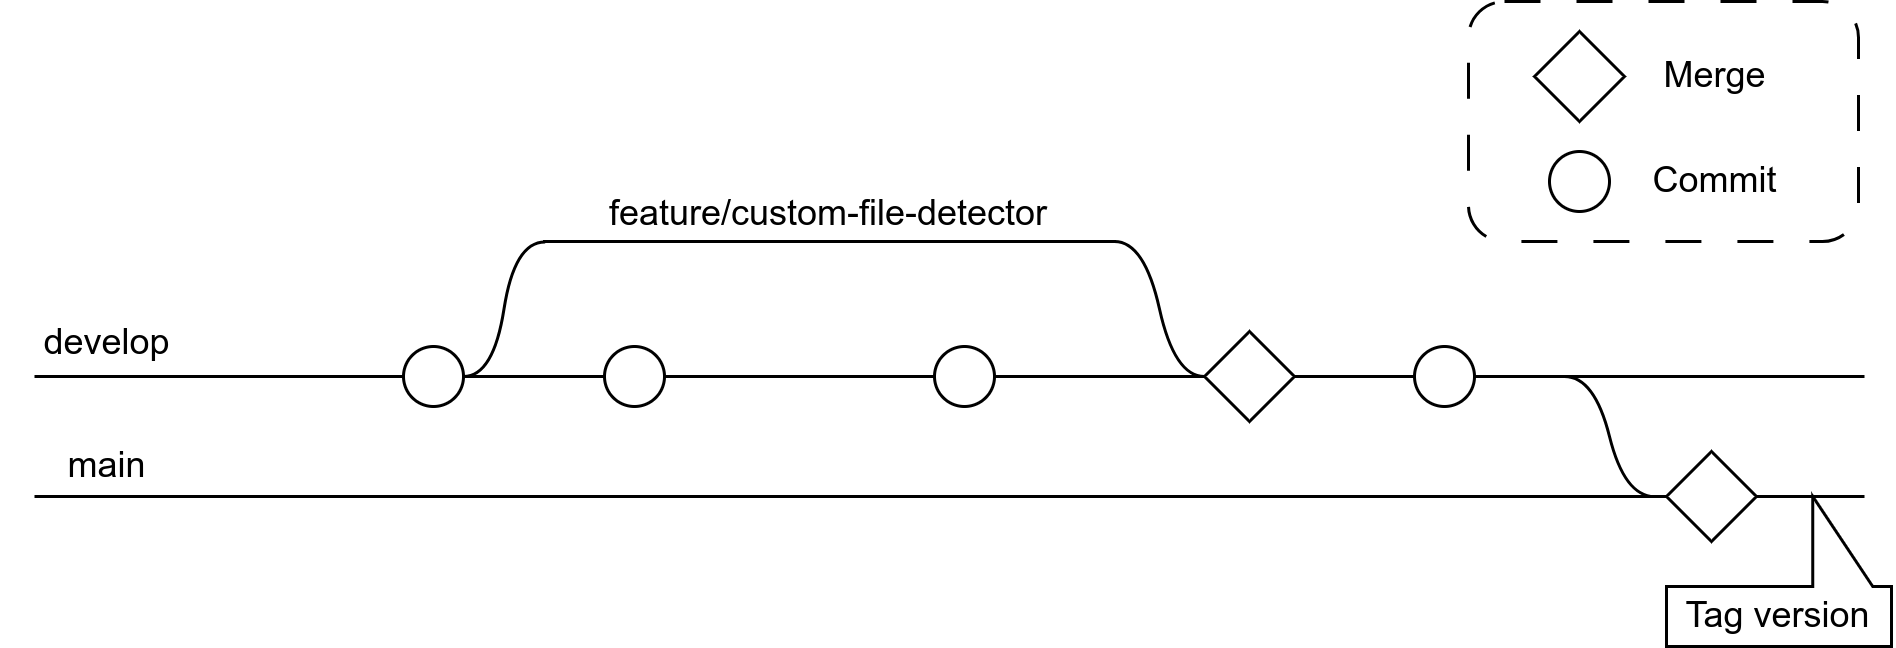
\includegraphics[width=\textwidth]{assets/git_branches_diagram.png}
    \caption{Struttura dei branch Git}
    \label{fig:git_branches_diagram}
\end{figure}